\section{Instruction Sets}

\subsection{More on Instruction Format}
\label{sec:instruction-format-extended}

\subsubsection{Arithmetic \& Logical Instructions}

\textbf{Arithmetic} operations treat operands as numbers and have to consider the sign
of the operands. Arithmetic shifts are equivalent to multiplication (left shift) or
division (right shift) by 2 with remainders shifted out. The new bits are filled with
sign bits on the left, and 0's on the right.

\textbf{Logical} operations treat operands as bit patterns. Logical shifts simply discard
the bits shifted out and replenish the new bits with 0's.

There are also \textbf{rotate} operations, which put the bits shifted out back into the
other end of the number.

\subsubsection{Procedures \& Function Calls}

A procedure consists of multiple instructions that are executed in sequence. Within
a procedure, instructions can be given to execute another procedure. For the CPU
to know where to go and where to return after the called procedure is done, the
return addresses need to be stored, which is done by a stack. The latest return
address will be at the top of the stack, and the CPU will pop it when it reaches
a return instruction.

\subsubsection{Instruction Operands}

In most applications, instructions either have three, two, one, or zero operands
(or addresses). Symbolically, they are represented as:

\begin{table}[H]
    \centering
    \begin{tabular}{|c|c|c|}
        \hline
        \textbf{\# of Operands} & \textbf{Symbolic Representation} & \textbf{Interpretation} \\
        \hline
        3 & \texttt{OP A, B, C} & \texttt{A} $\gets$ \texttt{B OP C} \\
        2 & \texttt{OP A, B} & \texttt{A} $\gets$ \texttt{A OP B} \\
        1 & \texttt{OP A} & \texttt{AC} $\gets$ \texttt{AC OP A} \\
        0 & \texttt{OP} & \texttt{T} $\gets$ \texttt{(T-1) OP T} \\
        \hline
    \end{tabular}
\end{table}

{\footnotesize Note: 
\texttt{AC} = accumulator, \texttt{T} = top of stack, \texttt{(T-1)} = second element of the stack
}

Instruction operands can either be in main memory or in registers.

\subsubsection{Registers}

\begin{itemize}
    \item \textbf{General Purpose Registers}: registers that can be used freely;
    \item \textbf{Dedicated Purpose Registers}: e.g. program counter (PC), instruction register (IR), stack pointer (SP), processor status word (PSW), flag register;
\end{itemize}

\subsubsection{Data Types}

Two types of data types: \begin{enumerate*}[label=\textbf{(\arabic*)}]
    \item Numeric (integer, floating point);
    \item Non-numeric (character, binary data).
\end{enumerate*}
The lengths are typically 8, 16, 32, or 64 bits.

For MIPS architecture (a family of reduced instruction set computer (RISC), not ARM or x86),
have 9 basic data types: \begin{enumerate*}[label=\textbf{(\arabic*)}]
    \item signed and unsigned bytes;
    \item signed and unsigned half-words;
    \item signed and unsigned words;
    \item double words;
    \item single-precision floating point (32 bits);
    \item double-precision floating point (64 bits)
\end{enumerate*}.

For ARM architecture, it supports datatypes of \begin{enumerate*}[label=\textbf{(\arabic*)}]
    \item byte (8 bits);
    \item half-word (16 bits); and
    \item word (32 bits)
\end{enumerate*} in length.
It only provides unsigned integers, nonnegative integers, and two's complement integers. 
The ARM architecture does not provide floating point hardware and they must be emulated in
software.

\subsection{Addressing Modes}

\begin{figure}[H]
    \centering
    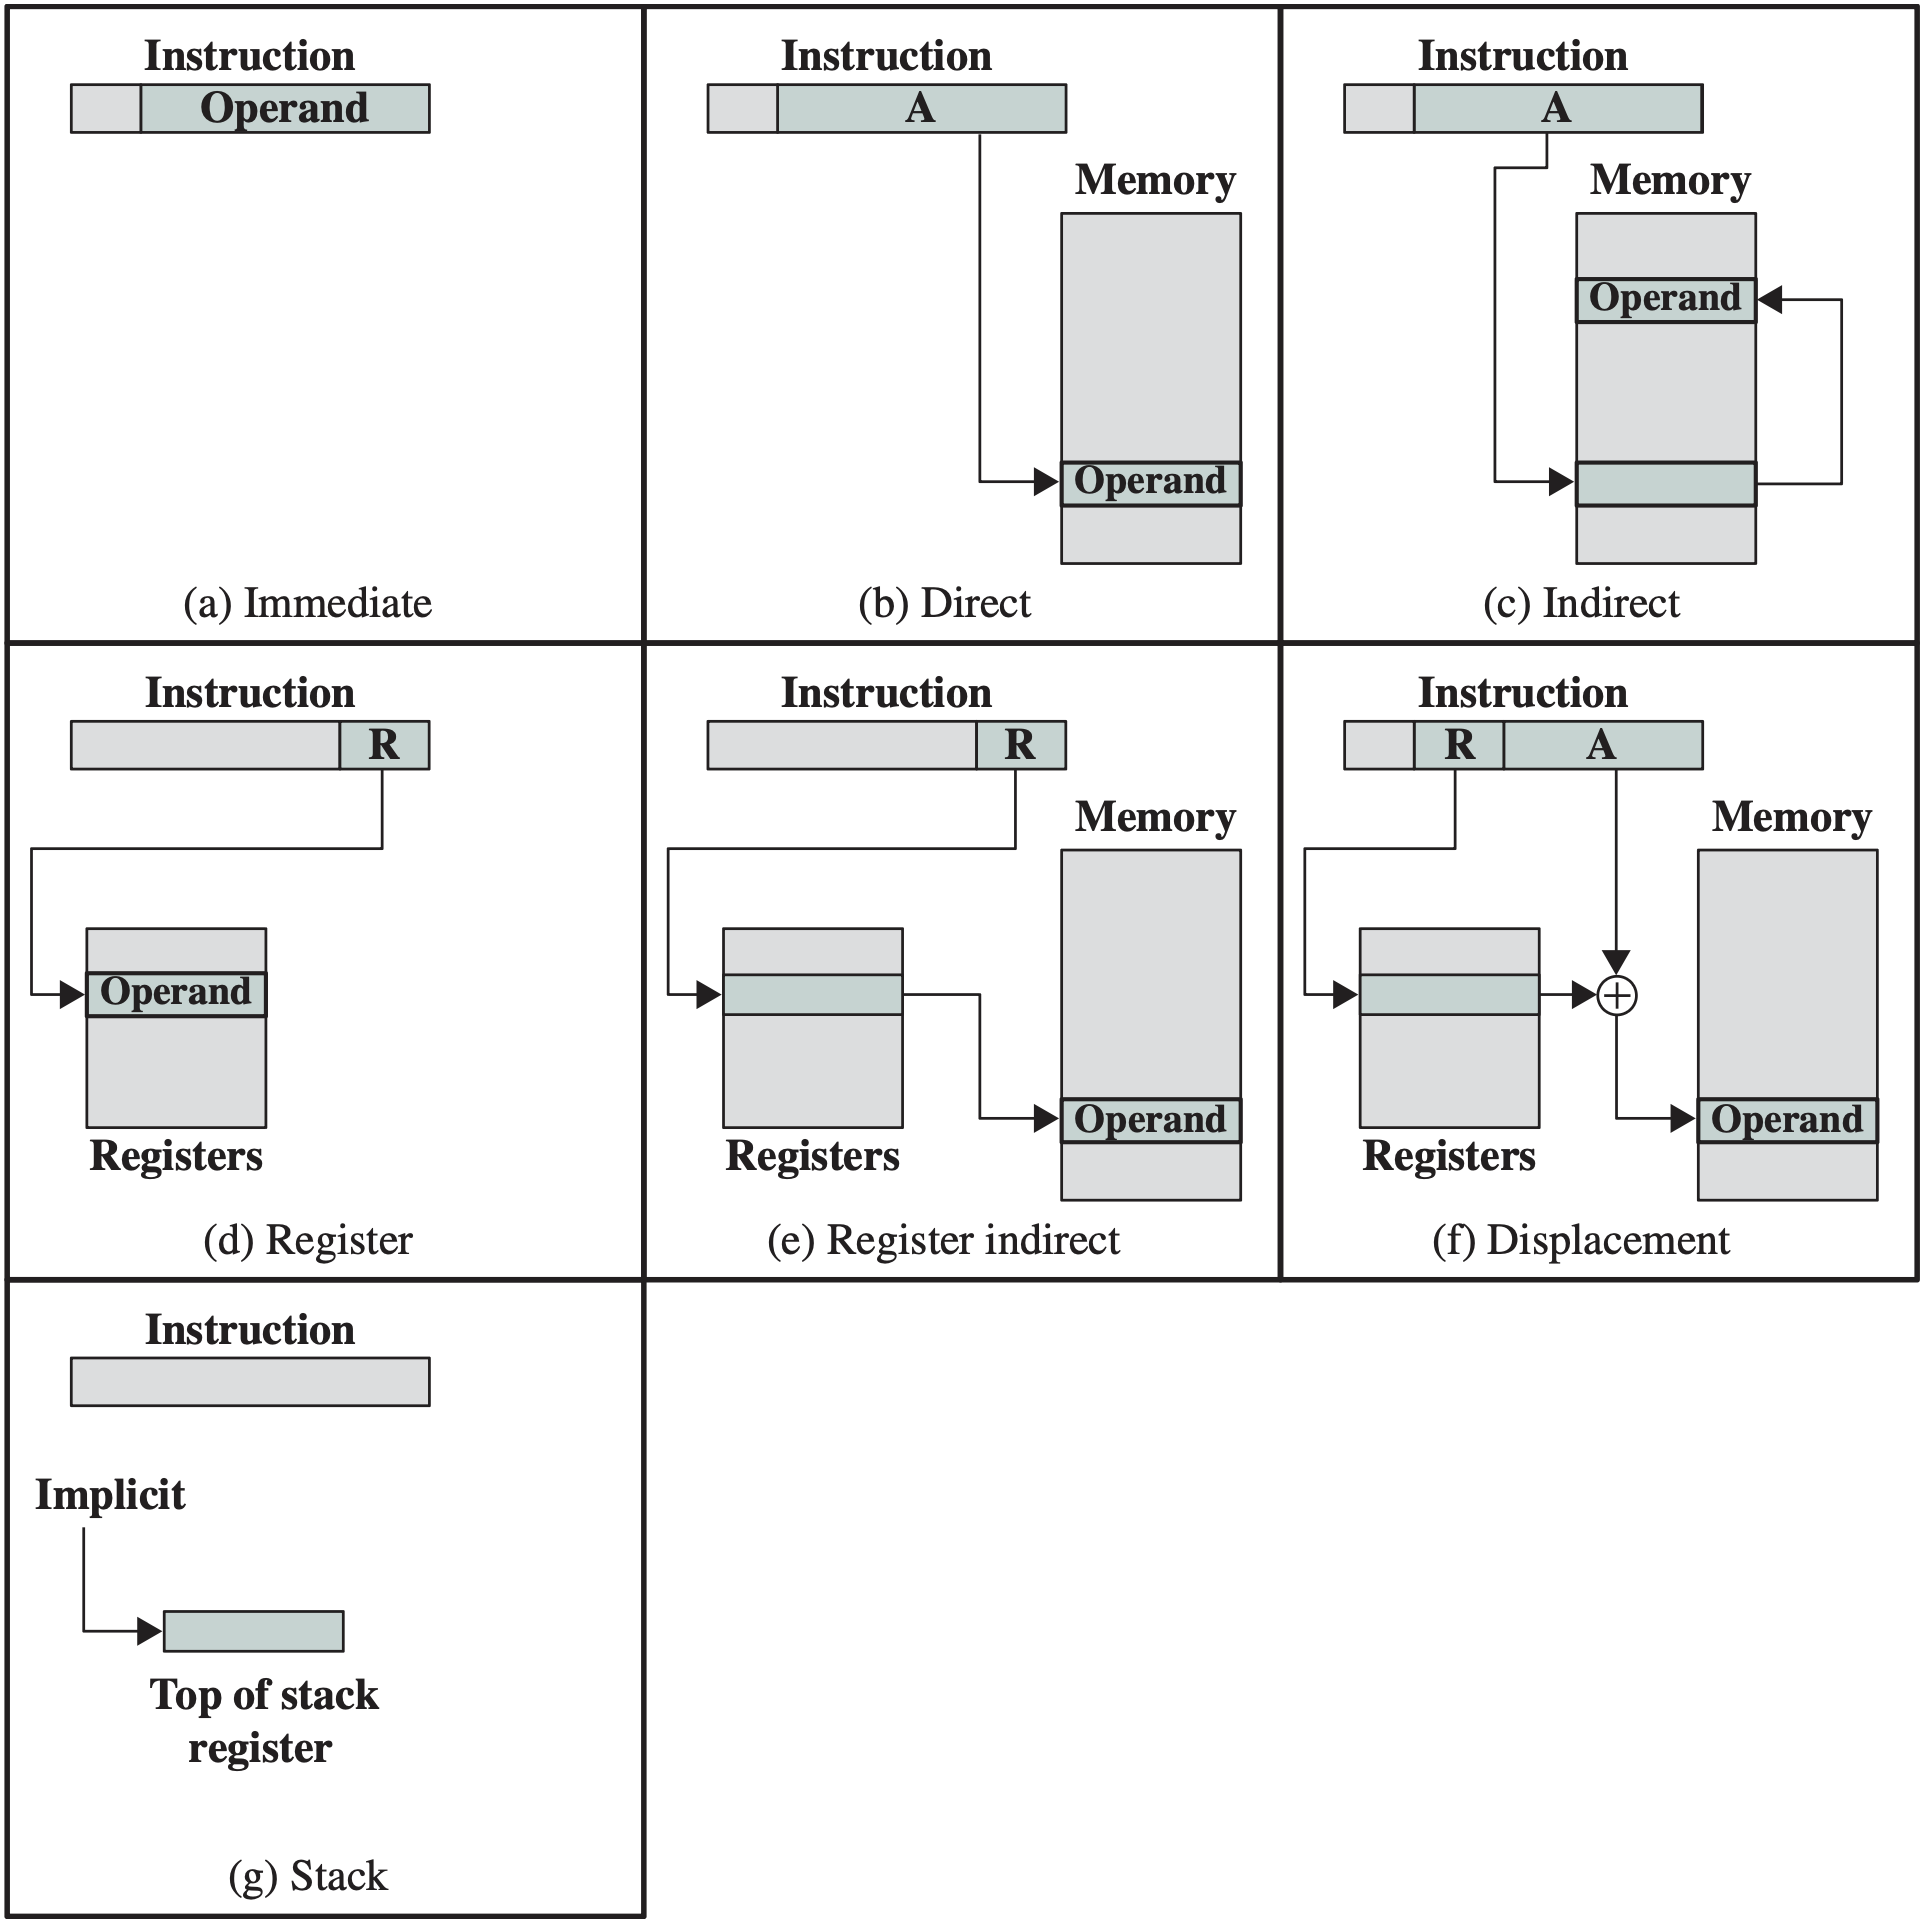
\includegraphics[width=0.8\textwidth]{chaps/instructions-sets/addressing-modes.png}
    \caption{Addressing Modes}
\end{figure}

\begin{remark}
    Notations used in this section:
    \texttt{A} = contents of an address (operand) field of an instruction;
    \texttt{R} = contents of an address field that refers to a register;
    \texttt{EA} = effective address (actual address) of the location where the referenced operand is stored;
    \texttt{(X)} = contents of memory location or register \texttt{X}.

    (The parenthesis notation is similar to a dereference operator of a pointer in C/C++.)
\end{remark}

\begin{multicols}{3}

\subsubsection{Immediate}

\begin{itemize}
    \item \textbf{Notation}: Operand $=$ \texttt{A}
    \item \textbf{Advantage}: No memory references needed.
    \item \raggedright\textbf{Disadvantage}: Limited operand magnitude.
\end{itemize}

\subsubsection{Direct}

\begin{itemize}
    \item \textbf{Notation}: \texttt{EA} $=$ \texttt{A}
    \item \textbf{Advantage}: Simple and increased operand magnitude.
    \item \textbf{Disadvantage}: Limited address space. (Range of memory addresses
        accessible to the instruction depends on the size of the address field.)
\end{itemize}

\columnbreak

\subsubsection{Indirect}

\begin{itemize}
    \item \textbf{Notation}: \texttt{EA} $=$ \texttt{(A)}
    \item \textbf{Advantage}: Increased address space.
    \item \textbf{Disadvantage}: Multiple memory references needed.
\end{itemize}

\subsubsection{Register}

\begin{itemize}
    \item \textbf{Notation}: \texttt{EA} $=$ \texttt{R}
    \item Similar to direct addressing, but the operand is in a register.
    \item \textbf{Advantage}: Fast access to operands.
    \item \textbf{Disadvantage}: Limited number of registers. (e.g. 32 registers in MIPS)
\end{itemize}

\columnbreak

\subsubsection{Register Indirect}

\begin{itemize}
    \item \textbf{Notation}: \texttt{EA} $=$ \texttt{(R)}
    \item Similar to indirect addressing, but the operand is in a register.
    \item \textbf{Advantage \& Disadvantage}: Same as indirect addressing.
\end{itemize}

\subsubsection{Displacement}

\begin{itemize}
    \item \textbf{Notation}: \texttt{EA} $=$ \texttt{A} $+$ \texttt{(R)}
    \item \textbf{Usage}: Accessing local variables or parameters in a function call,
        or accessing an array.
    \item Registers involved: PC, SP, and base pointer register.
    \item \textbf{Advantage}: Flexible.
    \item \textbf{Disadvantage}: Complex.
\end{itemize}

\end{multicols}

\subsubsection{Stack}

\begin{itemize}
    \item \textbf{Notation}: \texttt{EA} $=$ Top of Stack
    \item Uses the stack pointer register (SP). This is implied in the instruction.
    \item \textbf{Usage}: Mainly for \texttt{PUSH} and \texttt{POP} instructions.
    \item \textbf{Advantage}: No memory reference.
    \item \textbf{Disadvantage}: Limited applicability.
\end{itemize}

\subsection{Assembly Language Programming}

\begin{remark}

Assembly Language is very instruction set architecture (ISA) dependent. The language
differs from one architecture to another. This course focuses on a hypothetical
machine, with the following features:
\begin{itemize}
    \item Comments start with a \texttt{\#}\footnotemark and continue to the end of the line;
    \item Destination operands are on the \textbf{right} of the operands list;
    \item Instructions are case insensitive;
\end{itemize}

\end{remark}

\footnotetext{For using \LaTeX's \texttt{minted} package for syntex highlighting,
    the comment character in these notes will be ``\texttt{;}''.}

\subsubsection{Syntax}

\begin{definition}[Assembly Language Syntax]
    Each line of assembly language consists of:
    \begin{minted}[style=friendly]{asm}
        LABEL: OPERATION_MNEMONIC OPERAND_1, OPERAND_2, ..., OPERAND_N ; COMMENT
    \end{minted}
    \begin{itemize}
        \item \texttt{LABEL}: optional, used to identify a location in the program;
        \item \texttt{OPERATION\_MNEMONIC}: the operation to be performed;
        \item \texttt{OPERAND\_1, OPERAND\_2, ..., OPERAND\_N}: the operands for the operation;
        \item \texttt{COMMENT}: optional, used to explain the purpose of the instruction.
    \end{itemize}
\end{definition}

\subsubsection{Assembler Directives}

Like compiler directives in C/C++, assembly language also has assembler directives.
Assembler directives are for the assembler to perform an action or change a setting,
they are not translated into machine code. Assembler directives start with a dot.

\begin{table}[H]
    \centering
    \begin{tabularx}{\textwidth}{|l|*{1}{>{\RaggedRight\arraybackslash}X|}}
        \hline
        \textbf{Assembler Directive} & \textbf{Description} \\
        \hline
        \texttt{.DATA} & Adds the subsequent data to the data segment. \\
        \hline
        \texttt{.TEXT} & Adds the subsequent code to the text (program) segment. \\
        \hline
        \texttt{.GLOBAL NAME} & Makes \texttt{NAME} available to external files. \\
        \hline
        \texttt{.SPACE EXPRESSION} & Reserves spaces with the amount specified by the
        value of \texttt{EXPRESSION} in bytes. Reserved space is filled with 0's. \\
        \hline
        \texttt{.WORD VALUE\_1[, VALUE\_2, ...]} & Puts the values in successive memory
        locations.\\
        \hline
    \end{tabularx}
\end{table}

\subsubsection{Flow Control}

\begin{enumerate}

\item {\bfseries \texttt{IF...THEN...ELSE...} structure}
\begin{example}
    The following C/C++ code:
    \begin{minted}[style=friendly]{cpp}
    if (a[0] > a[1]) x = a[0];
    else x = a[1];
    \end{minted}
    is equivalent to the following assembly code:
\begin{minted}[style=friendly]{asm}
        .DATA   ; declares the data segment
a:      .WORD 1 ; a[0] = 1
        .WORD 3 ; a[1] = 3
x:      .WORD 4 ; x = 4
        .TEXT   ; declares the program segment
main:
        LD      [a], R8     ; load address of a into R8
        LD      0(R8), R9   ; load a[0] into R9 (displacement addressing)
        LD      4(R8), R10  ; load a[1] into R10 (displacement addressing)
        BGT     R9, R10, f1 ; if a[0] > a[1], branch to f1
        ST      R10, x      ; else: x = a[1]
        BR      f2
f1:     ST      R9, x       ; x = a[0]
f2:     RET                 ; return to the caller
\end{minted}
\end{example}

\item {\bfseries \texttt{FOR} loop}
\begin{example}
    The following C/C++ code:
    \begin{minted}[style=friendly]{cpp}
    a = 0;
    for (i = 0; i < 10; i++) a += i;
    \end{minted}
    is equivalent to the following assembly code:
\begin{minted}[style=friendly]{asm}
        .DATA   ; declares the data segment
a:      .WORD 0
        .TEXT
main:
        SUB     R8, R8, R8      ; prepare R8 = 0 as the counter
        LD      0xa, R9         ; constant 10 in R9 (hexadecimal)
        LD      0x1, R10        ; constant 1 in R10 for incrementing R8
        SUB     R11, R11, R11   ; use R11 as sum
L:      ADD     R11, R8, R11    ; R11 += R8
        ADD     R8, R10, R8     ; R8++
        BGT     R9, R8, L       ; branch to L if R9 (10) > R8 (counter)
        ST      R11, [a]
        RET
\end{minted}
\end{example}

\item {\bfseries \texttt{WHILE} loop} -- very similar to \texttt{FOR} loops.
\item {\bfseries Function calls}

Use \texttt{CALL} to make a function call, and \texttt{RET} to return from the function.
Input/return parameters are passed in registers and need to be documented by the developer.
If the function modifies some other registers, either document this behaviour, or use
\texttt{PUSH} and \texttt{POP} to save and restore the registers before and after the
function.
\begin{example}
    The following assembly code shows how to call a function \texttt{c\_mult} that
    multiplies two complex numbers.
    ($\Re(a\cdot b) = \Re(a)\cdot\Re(b) - \Im(a)\cdot\Im(b)$ and
    $\Im(a\cdot b) = \Re(a)\cdot\Im(b) + \Im(a)\cdot\Re(b)$)
\begin{minted}[style=friendly]{asm}
        .DATA
ar:     .WORD 1     ; Re(a) = 1 (real part of complex number a)
ai:     .WORD 5     ; Im(a) = 5 (imaginary part of complex number a)
br:     .WORD 2
bi:     .WORD 3
cr:     .WORD 0
ci:     .WORD 0
        .TEXT
main:
        LD      [ar], R8    ; Prepare parameters for c_mult
        LD      [ai], R9
        LD      [br], R10
        LD      [bi], R11
        CALL    c_mult      ; Call c_mult
        ST      R12, [cr]   ; Store the result
        ST      R13, [ci]
        RET
c_mult: 
        ; multiply two complex numbers
        ; input: R8 = Re(a), R9 = Im(a), R10 = Re(b), R11 = Im(b)
        ; output: R12 = Re(a*b), R13 = Im(a*b)
        PUSH    R14         ; use R14 as a temporary register
        MUL     R8, R10, R12
        MUL     R9, R11, R14
        SUB     R12, R14, R12
        MUL     R8, R11, R13
        MUL     R9, R10, R14
        ADD     R13, R14, R13
        POP     R14
        RET
\end{minted}
\end{example}

\end{enumerate}

\subsection{Operating System Support}

The operating system (OS) is a software that controls the execution of programs and
manages hardware resources. It allows a computer to be used efficiently and conveniently.

\textbf{Services provided by the OS}:
\begin{itemize}
    \item \textbf{Program Creation} -- through compilers, assemblers, editors, debuggers etc.
    \item \textbf{Program Execution} -- through loading programs into memory and preparing resources for the program
    \item \textbf{I/O Access} -- through providing a uniform I/O interface while the implementation is left to the OS
    \item \textbf{File System Management}
    \item \textbf{System Access} -- control access to system resources to prevent unauthorised users
    \item \textbf{Error Detection and Response}
    \item \textbf{Accounting} -- collecting usage statistics and monitoring performance parameters
\end{itemize}

\subsubsection{OS Protection Scheme}

Most OSs uses two modes of operation: \textbf{user mode} and \textbf{kernel mode}.
The CPU will execute in different modes to facilitate protection. Some OSs may use up
to four modes. Some resources are only accessible in kernel mode.

An OS is supposed to be well-tested, while bugs may exist in user programs.

OS functions are usually accessed via special entry points called \textbf{system calls}.
Upon a system call, the CPU will switch from user mode to kernel mode.

\subsubsection{Multitasking, Time Sharing \& Process Scheduling}

To fully utilise the CPU, the CPU is shared among multiple processes. Each process
is given a time slice to execute. When it uses up its time slice, the CPU will
suspend the execution and switch to another process.

The OS maintains a queue of processes in which the order of execution depends on
several factors, such as priority, waiting time, whether the process has used up
its time slice (i.e. CPU-bound jobs), the current system load, etc.

\subsection{Processor Organisation}

The processor executes instructions via moving data to the desired location and
performing data transformations/processing using the ALU. These operations are
controlled by the control signals generated by the control unit (CU).

\subsubsection{Data Movement and Transformation}

Recall the stages of an instruction execution cycle at Section \ref{lbl:instruction-execution-cycle}:
\begin{enumerate*}[label=\textbf{(\arabic*)}]
    \item IF, \item ID, \item CO, \item OF, \item EI, \item WO.
\end{enumerate*}
For modern processors, only \texttt{LD} and \texttt{ST} instructions are related to memory operands
and they do not need the \texttt{EI} stage. Other instructions usually do not need the \texttt{CO} stage.

\begin{example}
    Suppose the instruction \texttt{ADD A, B, C} uses direct addressing mode, and A, B, and C
    are supplied in the words following the instruction. Write down the involved data movement.

    \begin{multicols}{2}
        \ttfamily
        \textbf{; IF - Instruction Fetch} 

        MAR $\gets$ PC \\
        PC $\gets$ PC + 4 ; PC now points to A\\
        IR $\gets$ mem[MAR]

        \textbf{; ID - Instruction Decode}

        \textbf{; CO(A) - Calculate Operand (A)} 

        MAR $\gets$ PC ; MAR has address to address of A \\
        PC $\gets$ PC + 4 ; PC now points to B \\
        MBR $\gets$ mem[MAR] ; MBR has the address of A

        \textbf{; FO(A) - Fetch Operand (A)} 

        MAR $\gets$ MBR ; MAR has the address of A \\
        MBR $\gets$ mem[MAR] ; MBR has the value of A \\
        ALU\_IN\_1 $\gets$ MBR ; ALU\_IN\_1 has the value of A

        \textbf{; CO(B) - Calculate Operand (B)} 

        MAR $\gets$ PC ; MAR has address to address of B \\
        PC $\gets$ PC + 4 ; PC now points to C \\
        MBR $\gets$ mem[MAR] ; MBR has the address of B

        \textbf{; FO(B) - Fetch Operand (B)} 

        MAR $\gets$ MBR ; MAR has the address of B \\
        MBR $\gets$ mem[MAR] ; MBR has the value of B \\
        ALU\_IN\_2 $\gets$ MBR ; ALU\_IN\_2 has the value of B

        \textbf{; EI - Execute Instruction} 

        ALU\_OUT $\xleftarrow{\texttt{ALU}}$ ALU\_IN\_1 + ALU\_IN\_2

        \textbf{; WO - Write Operand} 

        MAR $\gets$ PC ; MAR has address to address of C \\
        PC $\gets$ PC + 4 ; PC points to next instruction \\
        MBR $\gets$ mem[MAR] ; MBR has the address of C \\
        MAR $\gets$ MBR ; MAR has the address of C \\
        MBR $\gets$ ALU\_OUT ; MBR has the value of A + B \\
        mem[MAR] $\gets$ MBR ; Writes the result to C
    \end{multicols}
\end{example}

\subsection{Reduced Instruction Set Computer (RISC) Architecture}